\subsection{Bioinformatics Analysis of Bovine IFITs} \label{subsec:Bioinformatics Analysis of Bovine IFITs}
lorem ipsum

\subsubsection{RNA-Seq Analysis}
\myparagraph{Validation by analysing bRSV RNAseq dataset} \label{Validation by analysing bRSV RNAseq dataset}
Describe data: \newline
asdasdas \newline
Data showing that bIFITs are not differentially expressed in cells infected with dSH bRSV.

This is a dataset that was present in Dalan`s group. Comparing responses at 16 and 40 HPI between WT bRSV vs Mock and dSH bRSV vs Mock. The dataset was previously analysed by a bioinformatician in Pirbright which yield 0 differentially expressed host genes. He however included viral genes in the analysis, which I assume affected the adjusted p values of the host genes due to the relative viral genes abundance. We tried to get in touch with him to discuss this but after several emails got no response. The re-analysis was done on raw annotated count data which had viral transcripts removed. Original analysis was done using EdgeR package, my re-analysis was with DESeq2 (both are valid way of doing DE analysis, EdgeR is more modular and harder to use).

All 4 volcano plots, showing bi1-5 and bmx1, regardless where they are

\begin{figure}
    \centering
    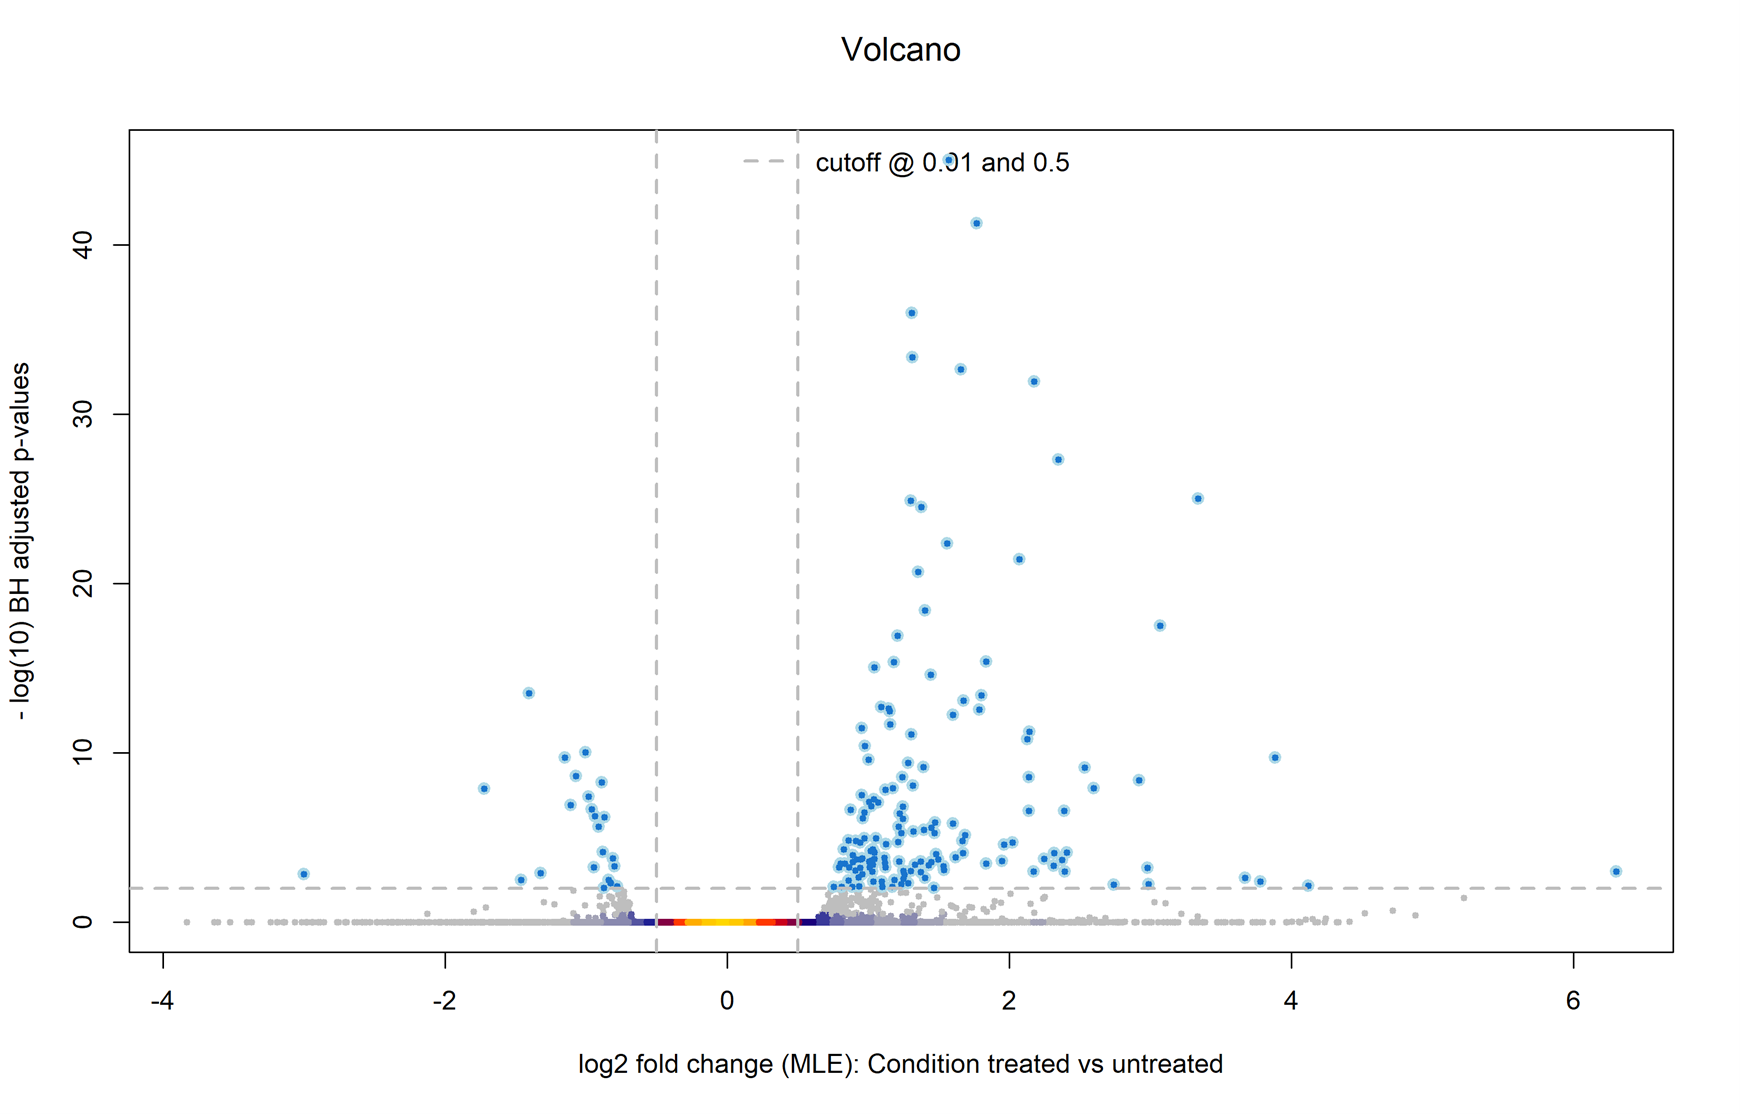
\includegraphics[width=1\linewidth]{07. Chapter 2//Figs/14. rnaseq volcano.png}
    \caption[Volcano plot of DE genes in WT vs Mock 40 HPI.]{\textbf{Volcano plot of DE genes in WT vs Mock 40 HPI.} asdf asdf asdf asdf asdf asdf asdf asdf asdf }
    \label{fig:Volcano plot of DE genes in WT vs Mock 40 HPI}
\end{figure}

\begin{figure}
    \centering
    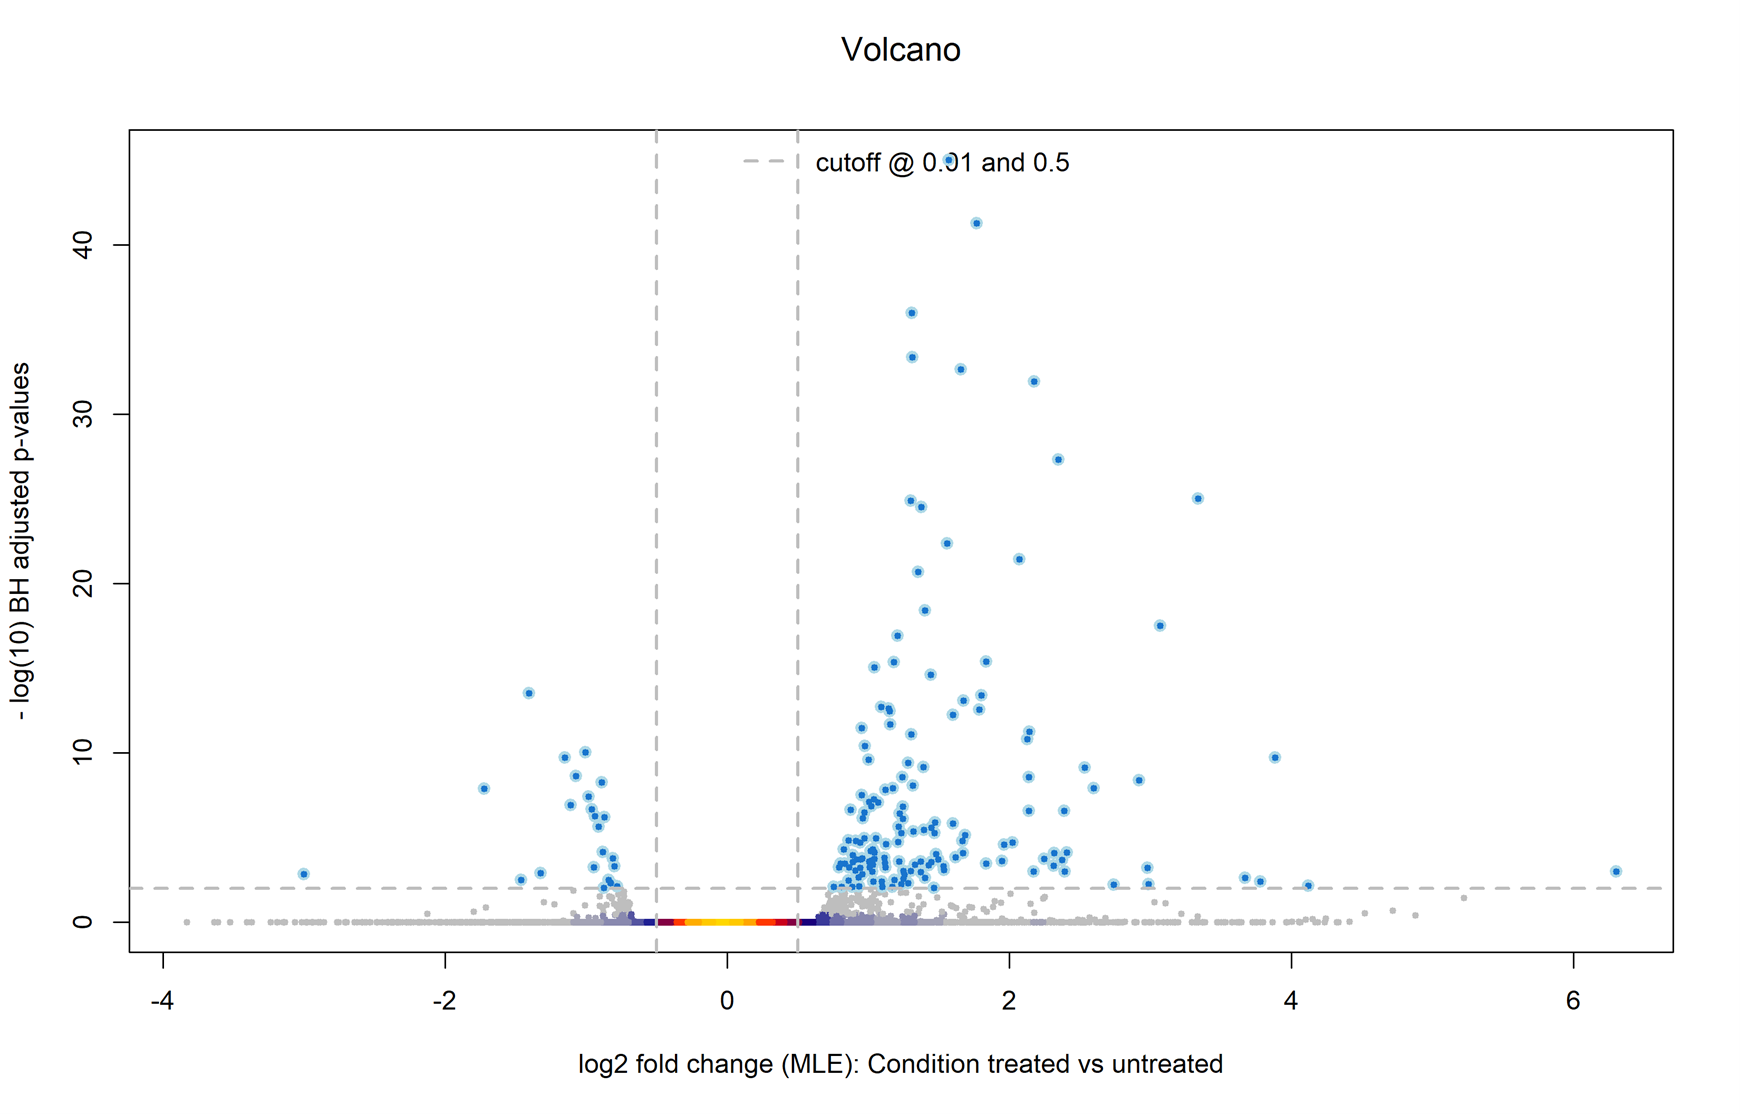
\includegraphics[width=1\linewidth]{07. Chapter 2//Figs/14. rnaseq volcano.png}
    \caption{Enter Caption}
    \label{fig:volcano2}
\end{figure}

afterwards i would do a paragraph of the analysis as I did it so why not

\subsubsection{Meta-Analysis}
lorem ipsum

\subsubsection{Summary}
lorem ipsum